\fig{fv:m1:sheet}{面电流的自场两侧反向，取平均才消去自场}{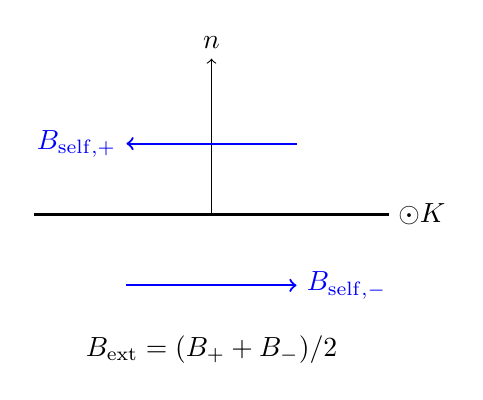
\begin{tikzpicture}[scale=.9]
\draw[very thick](-2.5,0)--(2.5,0);\node[right]at(2.5,0){$\odot K$};\draw[->](0,0)--(0,2.2)node[above]{$\bm n$};
\draw[->,blue,thick](1.2,1)--(-1.2,1)node[left]{$\bm B_{\rm self,+}$};
\draw[->,blue,thick](-1.2,-1)--(1.2,-1)node[right]{$\bm B_{\rm self,-}$};
\node at(0,-1.9){$\bm B_{\rm ext}=(\bm B_++\bm B_-)/2$};\end{tikzpicture}}
图\ref{fv:m1:sheet}取面电流向纸外、正法线向上，右手关系给上方自场向左、下方向右。叠加同一个平滑外场后，两侧总场之差保留自场的跳变，平均值则消去这对反向贡献。计算面本身受力所需的正是剩下的外场，而非任意一侧总场。这把环路的边界关系与薄层机械受力联系起来，也说明用层间总场求单层力为何容易多算一倍。
